%GiG
\documentclass{beamer} 
\usetheme{Copenhagen}
\setbeamertemplate{navigation symbols}{}
\setbeamertemplate{headline}{}
\DeclareMathOperator*{\argmax}{arg\,max}

\usepackage{hyperref}
\definecolor{azure}{rgb}{0.0, 0.5, 1.0}
%\newcommand{\tblue}[1]{\textcolor{blue}{#1}}
\newcommand{\tblue}[1]{{\Large {\textcolor{azure}{#1}}}}
\newcommand{\hred}[1]{{\textcolor{red}{#1}}}

\title[Saravanan Thirumuruganathan] 
{Lecture 2: Divide\&Conquer Paradigm, Merge sort and Quicksort}

\author[CSE 5311] 
{Instructor: Saravanan Thirumuruganathan}

\date[] 

\begin{document}

\begin{frame}
  \titlepage
\end{frame}

%\begin{frame}{Outline}
%  \tableofcontents
%  % You might wish to add the option [pausesections]
%\end{frame}

\section{Outline}

\begin{frame}
\frametitle {Outline}
\begin{enumerate}
\item Divide and Conquer
\item Merge sort
\item Quick sort
\end{enumerate}
\end{frame}

\begin{frame}{In-Class Quizzes}
\begin{itemize}
\item {\Large {\bf URL:}} {\LARGE \bf \url{http://m.socrative.com/}} 
\item {\Large {\bf Room Name:} {\LARGE \bf 4f2bb99e}}
\end{itemize}
\end{frame}

\section{Divide and Conquer Paradigm}

\begin{frame}{Divide And Conquer Paradigm}
\begin{itemize}
\item D\&C is a popular algorithmic technique
\item Lots of applications
\item Consists of three steps:
\begin{enumerate}
    \item {\bf Divide} the problem into a number of sub-problems
    \item {\bf Conquer} the sub-problems by solving them {\em recursively}
    \item {\bf Combine} the solutions to sub-problems into solution for original problem 
\end{enumerate}
\end{itemize}
\end{frame}


\begin{frame}{Divide And Conquer Paradigm}

\tblue{When can you use it?}
\begin{itemize}
\item The sub-problems are easier to solve than original problem
\item The number of sub-problems is {\bf small}
\item Solution to original problem can be obtained easily, once the sub-problems are solved
\end{itemize}
\end{frame}


\begin{frame}{Recursion and Recurrences}
\begin{itemize}
\item Typically, D\&C algorithms use {\bf recursion} as it makes coding simpler
\item Non-recursive variants can be designed, but are often slower
\item If all sub-problems are of equal size, can be analyzed by the recurrence equation 
$$ T(n) = a T(\frac{n}{b}) + D(n) + C(n)$$
\item $a$: number of sub-problems to solve 
\item $b$: how fast the problem size shrinks
\item $D(n)$: time complexity for the divide step
\item $C(n)$: time complexity for the combine step
\end{itemize}
\end{frame}

\begin{frame}{D\&C Approach to Sorting}

\tblue{How to use D\&C in Sorting?}
\begin{itemize}
\item Partition the array into sub-groups
\item Sort each sub-group recursively
\item Combine sorted sub-groups if needed
\end{itemize}
\end{frame}

\section{Merge Sort}
\begin{frame}{Why study Merge Sort?}
\begin{itemize}
\item One of the simplest and efficient sorting algorithms
\item Time complexity is $\Theta(n \log n)$ (vast improvement over Bubble, Selection and Insertion sorts)
\item Transparent application of D\&C paradigm
\item Good showcase for time complexity analysis
\end{itemize}
\end{frame}


\begin{frame}{Merge Sort}

\tblue{High Level Idea :}
\begin{itemize}
\item Divide the array into two {\bf equal} partitions - left and right (ignore edge cases for now)
\item Sort left partition recursively
\item Sort right partition recursively
\item Merge the two sorted partitions into the output array
\end{itemize}
\end{frame}


\begin{frame}[fragile]{Merge Sort Pseudocode}

\tblue{Pseudocode:}
\begin{verbatim}
MergeSort(A, p, r):
    if p < r:
        q = (p+r)/2
        Mergesort(A, p , q)
        Mergesort(A, q+1, r)
        Merge(A, p, q, r)
\end{verbatim}
\end{frame}


\begin{frame}{Merge Sort - Divide\footnote{\url{http://web.stanford.edu/class/cs161/slides/0623_mergesort.pdf}}}
\begin{center}
    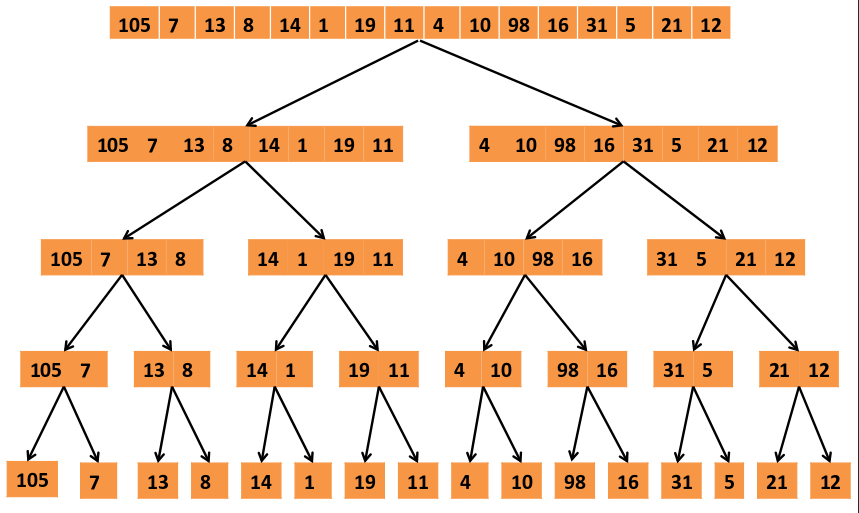
\includegraphics[scale=0.38]{mergeSortRecursion.png}
\end{center}
\end{frame}


\begin{frame}{Merge Sort - Combine\footnote{\url{http://web.stanford.edu/class/cs161/slides/0623_mergesort.pdf}}}
\begin{center}
    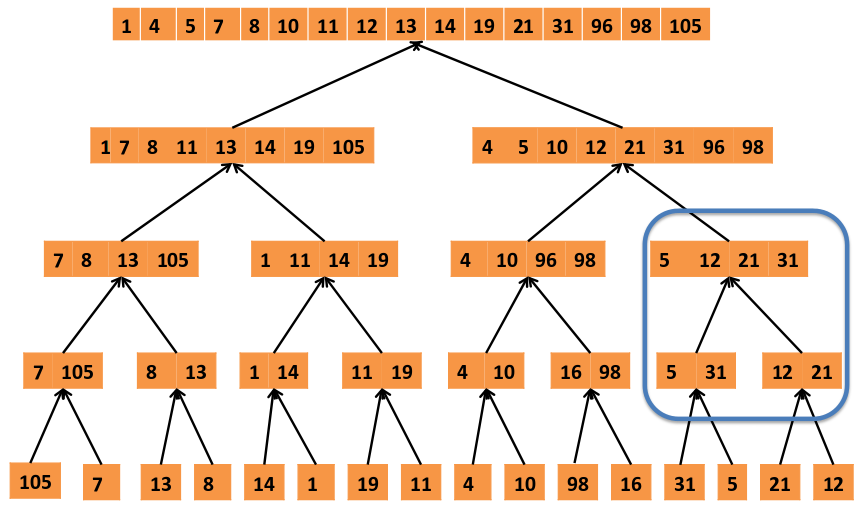
\includegraphics[scale=0.36]{mergeSortMerge.png}
\end{center}
\end{frame}


\begin{frame}{Merging Two Sorted Lists\footnote{\url{http://web.stanford.edu/class/cs161/slides/0623_mergesort.pdf}}}
\begin{center}
    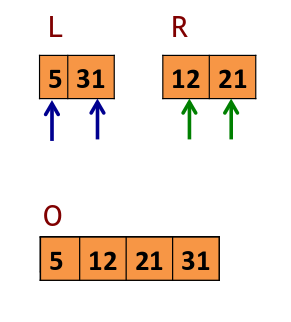
\includegraphics[scale=0.5]{mergeListExample.png}
\end{center}
\end{frame}


\begin{frame}{Merging Two Sorted Lists}
\begin{center}
    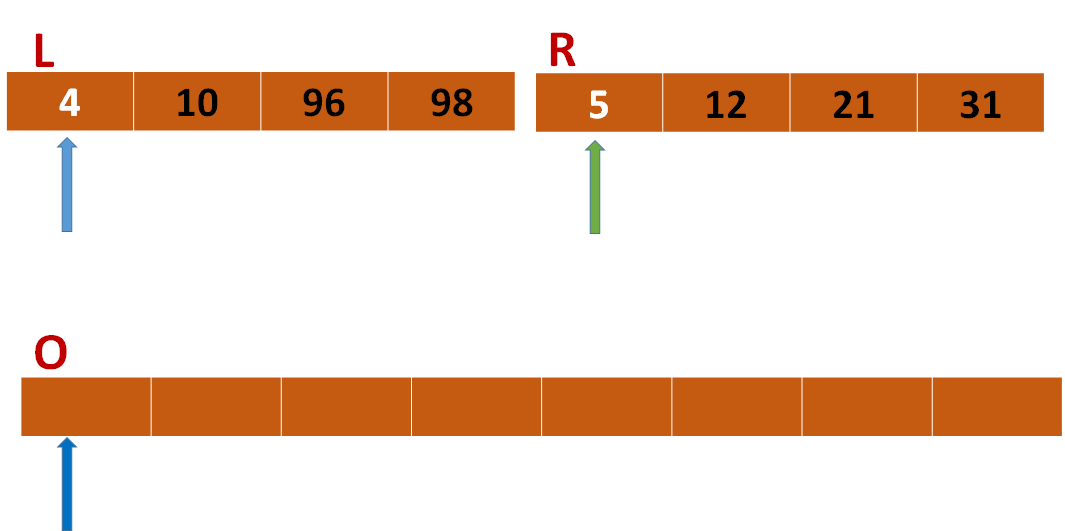
\includegraphics[scale=0.4]{mergeStep1.png}
\end{center}
\end{frame}




\begin{frame}{Merging Two Sorted Lists}
\begin{center}
    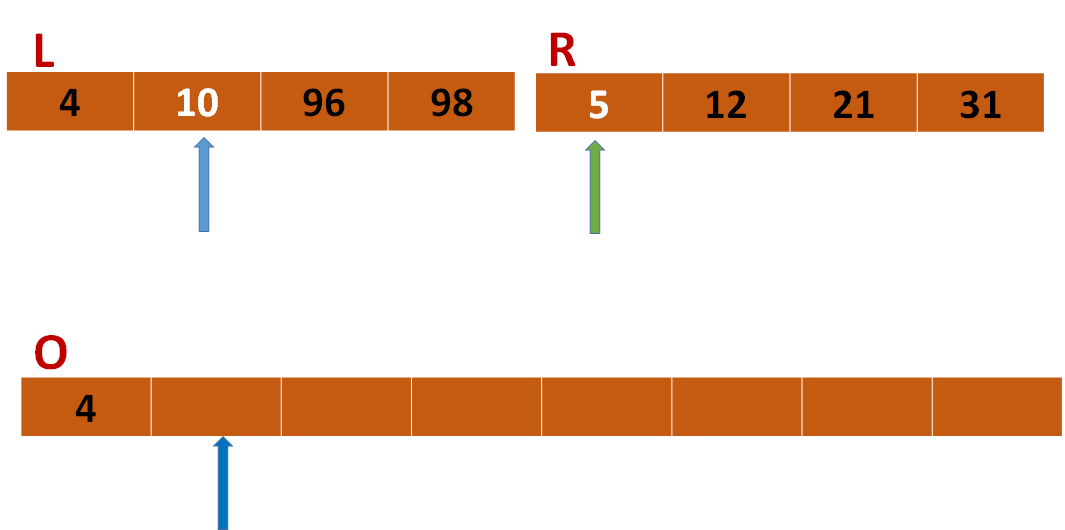
\includegraphics[scale=0.4]{mergeStep2.png}
\end{center}
\end{frame}




\begin{frame}{Merging Two Sorted Lists}
\begin{center}
    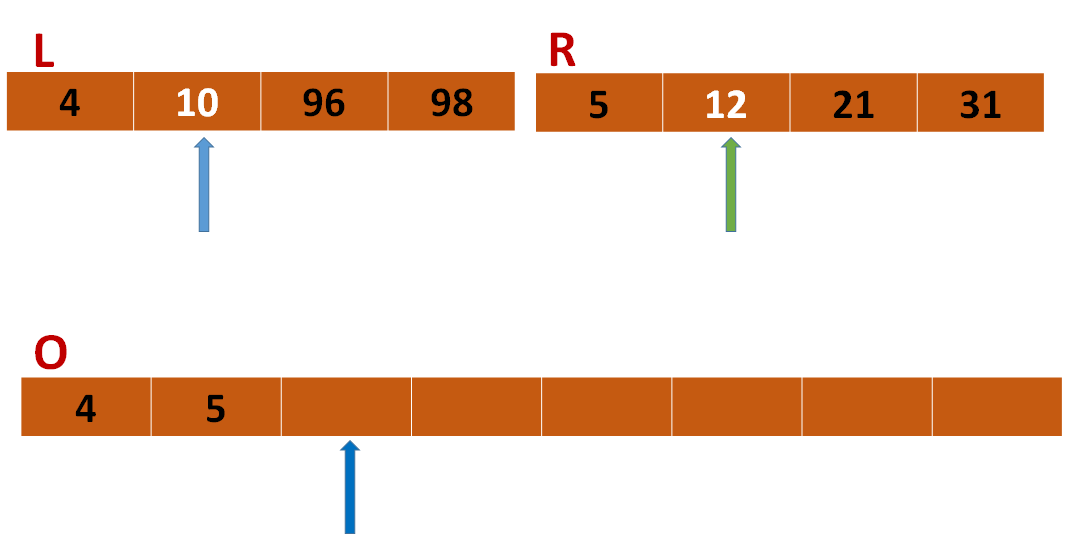
\includegraphics[scale=0.4]{mergeStep3.png}
\end{center}
\end{frame}




\begin{frame}{Merging Two Sorted Lists}
\begin{center}
    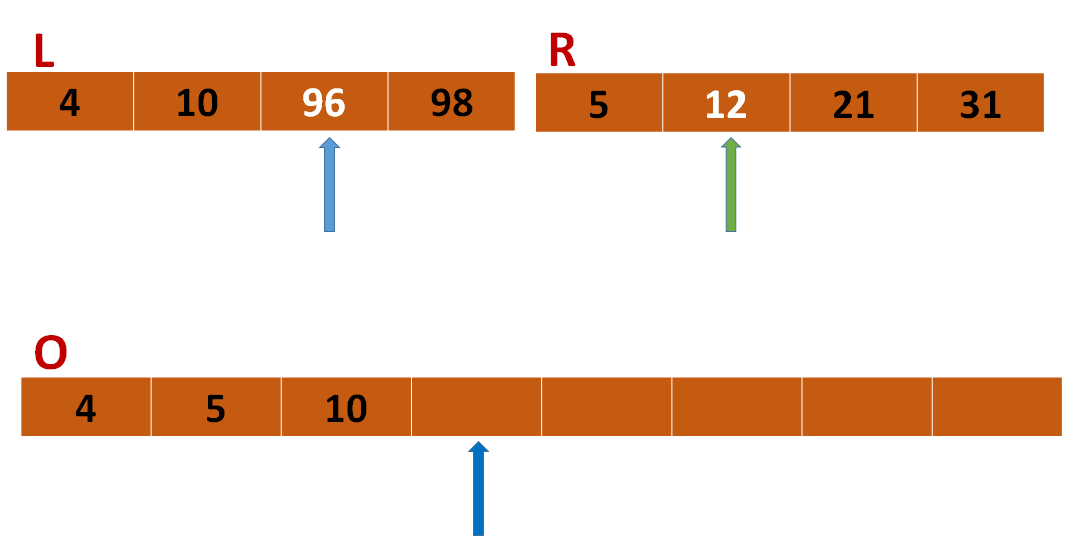
\includegraphics[scale=0.4]{mergeStep4.png}
\end{center}
\end{frame}




\begin{frame}{Merging Two Sorted Lists}
\begin{center}
    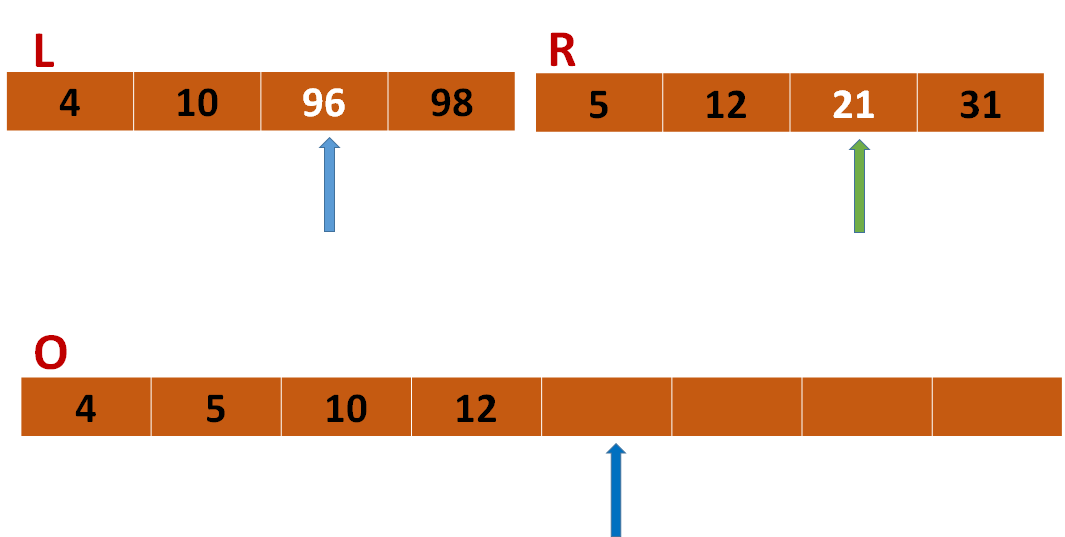
\includegraphics[scale=0.4]{mergeStep5.png}
\end{center}
\end{frame}




\begin{frame}{Merging Two Sorted Lists}
\begin{center}
    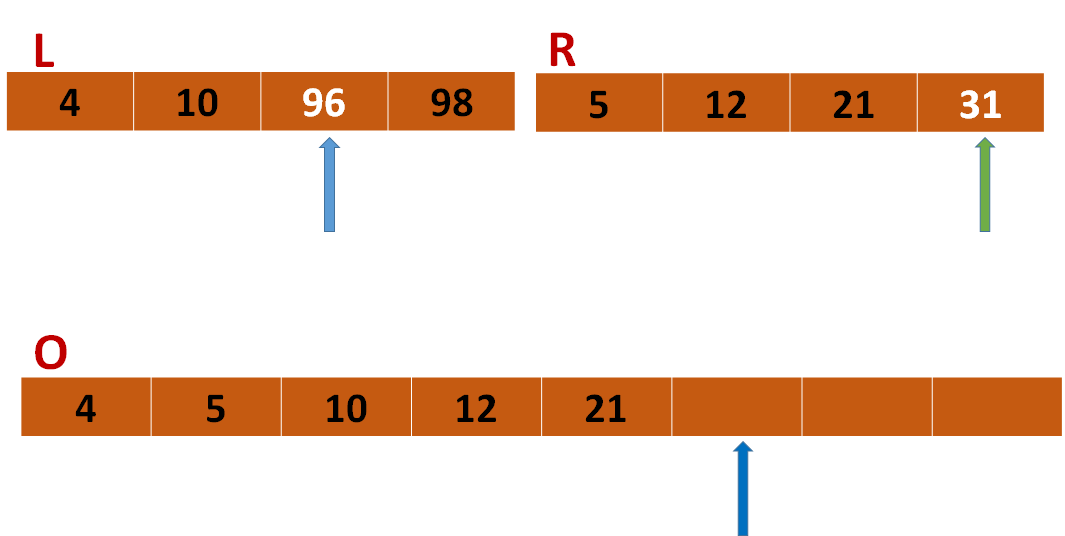
\includegraphics[scale=0.4]{mergeStep6.png}
\end{center}
\end{frame}




\begin{frame}{Merging Two Sorted Lists}
\begin{center}
    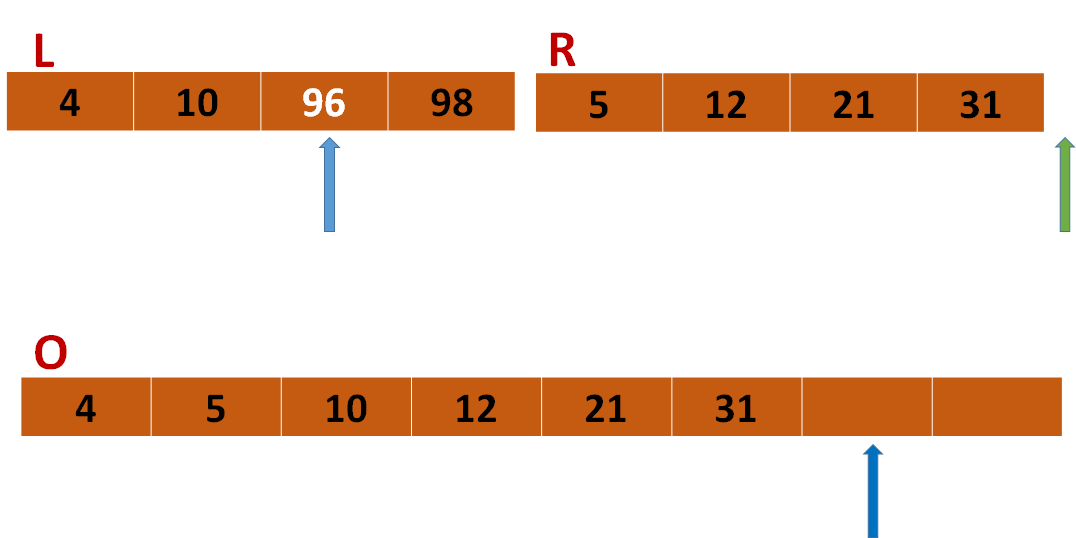
\includegraphics[scale=0.4]{mergeStep7.png}
\end{center}
\end{frame}




\begin{frame}{Merging Two Sorted Lists}
\begin{center}
    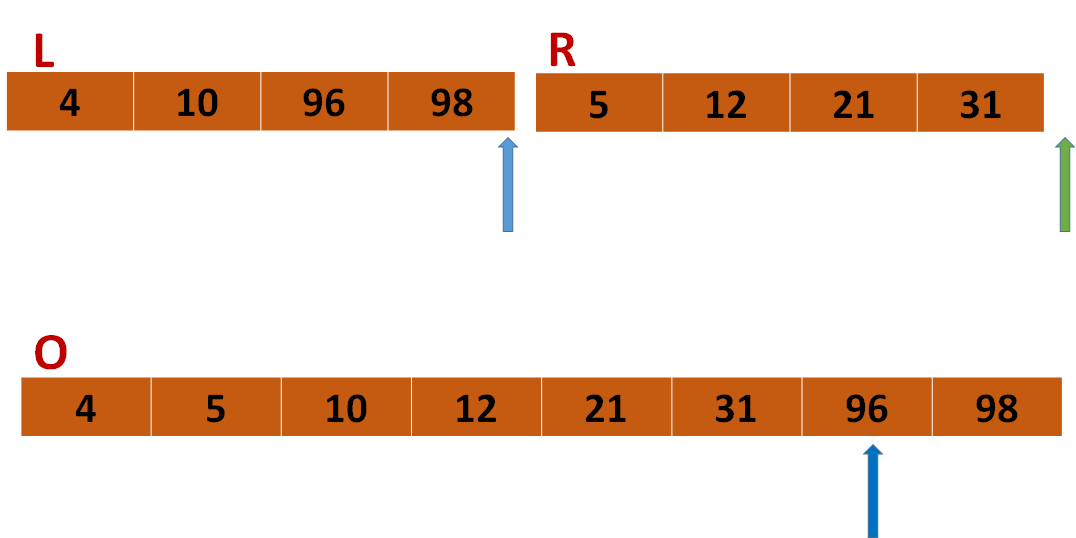
\includegraphics[scale=0.4]{mergeStep8.png}
\end{center}
\end{frame}


\begin{frame}[fragile]{Merging Two Sorted Lists}

\tblue{Merge Pseudocode:}

\begin{verbatim}
Merge(A,B,C):
    i = j = 1
    for k = 1 to n:
        if A[i] < B[j]:
            C[k] = A[i]
            i = i + 1
        else: (A[i] > B[j])
            C[k] = B[j]
            j = j + 1
\end{verbatim}
\end{frame}




\begin{frame}{Analyzing Merge Sort: Master Method}

\tblue{Quiz!}
\begin{itemize}
\item General recurrence formula for D\&C is  $T(n) = a T(\frac{n}{b}) + D(n) + C(n)$
\item What is $a$?
\item What is $b$?
\item What is $D(n)$?
\item What is $C(n)$?
\end{itemize}
\end{frame}


\begin{frame}{Analyzing Merge Sort: Master Method}

\tblue{Quiz!}
\begin{itemize}
\item General recurrence formula for D\&C is  $$T(n) = a T(\frac{n}{b}) + D(n) + C(n)$$
\item $a=2$, $b=2$
\item $D(n)=O(1)$
\item $C(n)=O(n)$
\item Combining, we get: $$T(n) = 2T(\frac{n}{2}) + O(n)$$
\item Using Master method, we get $T(n) = O(n \log n)$
\item If you are picky, $T(n) = T(\lceil \frac{n}{2} \rceil) + T(\lfloor \frac{n}{2} \rfloor) + O(n)$
\end{itemize}
\end{frame}


\begin{frame}{Analyzing Merge Sort: Recursion Tree\footnote{CLRS Book}}
\begin{center}
    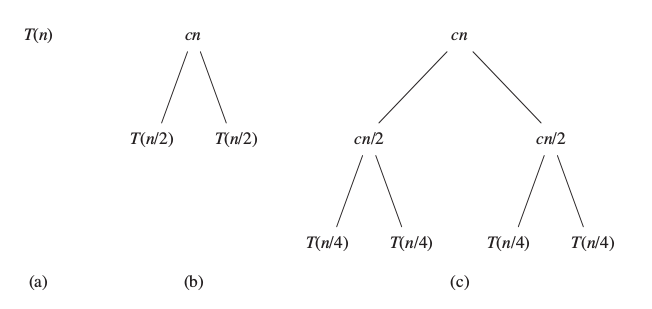
\includegraphics[scale=0.5]{mergeSortRecursionTree1.png}
\end{center}
\end{frame}



\begin{frame}{Analyzing Merge Sort: Recursion Tree\footnote{CLRS Book}}
\begin{center}
    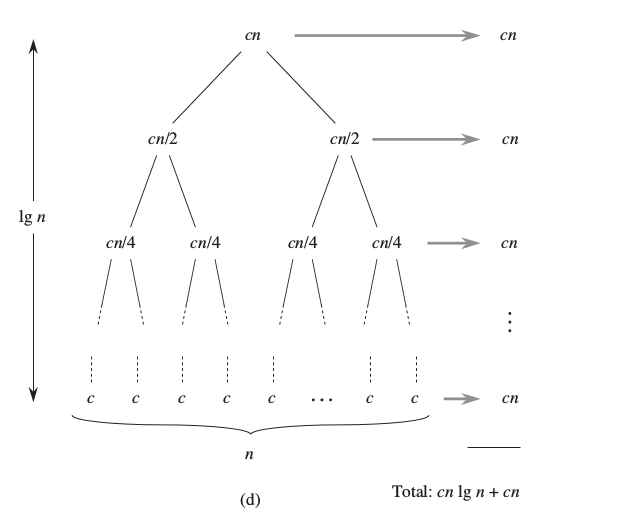
\includegraphics[scale=0.4]{mergeSortRecursionTree2.png}
\end{center}
\end{frame}


\begin{frame}{Merge Sort Vs Insertion Sort}
\begin{itemize}
\item Merge Sort is very fast in general ($O(n \log n)$) than Insertion sort ($O(n^2)$)
\item For ``nearly'' sorted arrays, Insertion sort is faster
\item Merge sort has $\hred{\Theta}(n \log n)$ (i.e. both best and worst case complexity is $n \log n$
\item Overhead: recursive calls and extra space for copying
\item Insertion sort is in-place and adaptive
\item Merge sort is easily parallizable 
\end{itemize}
\end{frame}

%\begin{frame}{QuickSort}
%\begin{center}
%    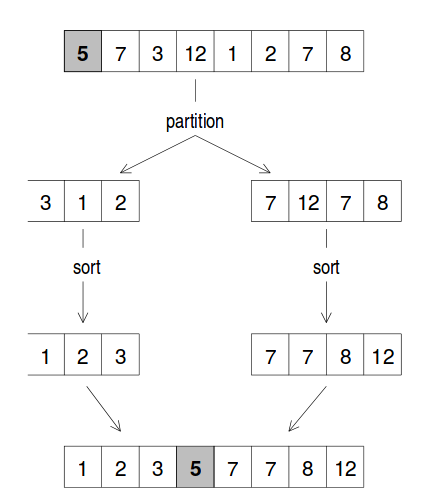
\includegraphics[scale=0.4]{quickSortHighLevelExample.png}
%\end{center}
%\end{frame}

%\begin{frame}{GiG}
%\begin{itemize}
%\item GiG
%\end{itemize}
%\end{frame}


%\begin{frame}{Sorting in the Real World}
%\begin{itemize}
%\item Sorting is a fundamental problem with intense ongoing research
%\item No single best algorithm - Merge, Quick, Heap, Insertion sort all excel in some scenarions
%\item Most programming languages implement sorting via tuned QuickSort (e.g. Java 6 or below) or 
%a combination of Merge Sort and Insertion sort (Python, Java 7, Perl etc).
%\end{itemize}
%\end{frame}

%\begin{frame}{Summary}

%\tblue{Major Topics:}
%\begin{itemize}
%\item TBD
%\end{itemize}
%\end{frame}


\end{document}

